\chapter{Introduction}
The mammalian brain is one of the most complex biological structures known to man and it has been the center of intense study for centuries.  A rather striking feature of the brain is just how reliably its gross anatomy is preserved across individuals and generations.  The fact that complex neuroanatomy is faithfully preserved in such a manner requires that the mechanisms through which brain structures are created in development and maintained throughout life are rather stereotyped as well.  Much work has been done, principally in the last half of the last century, in an attempt delineate the precise mechanisms of neural development.  Two general classes of neural development models have emerged from this work.
	The first class of models for neural development are based on activity dependent mechanisms.  Under these models, developing neural systems exhibit a profound period of early and exuberant connectivity.  Neurons make many early connections, some of which are ultimately appropriate and are maintained.  Other inappropriate connections are pruned away in a period of neuronal refinement that follows initial connection events. Neural connections under these models are either strengthened in the case of appropriate connections or weakened in the case of inappropriate connections through synaptic re-weighting based on activity patterns in the system.  Under these models the driving force for proper neural development is patterned activity  (LeVay et al., 1978). External and internal environmental influences on the system hold sway and have a dramatic effect on the structure and function of the brain.  The systematic replication of gross neuronal structure across individuals is thus explained by stereotyped environmental influences on the developing nervous system.
	The second class of models for neural development are based on molecular cues.  Under these models, there is a molecular blueprint that defines the pattern of neural connections.  In stark contrast to activity dependent sorting of neural connections, connections are precise at their onset under these models. Here, the structure of the brain is set forth at the most fundamental level.  Genetically encoded molecular cues guide axons and dendrites in the developing nervous system to their appropriate targets and there is little need for large-scale rewiring of the system (Sperry, 1963).  Environmental influences on the brain are marginalized to a role in which they only fine tune the structure set forth by genetically encoded molecular cues.  The striking reliability of gross neuronal structures is thus explained by a preservation of the genetic material which drives the formation of the brain. 
	One of the first neural systems studied in great detail was the visual system (Hubel, 1982).  The visual system of binocular mammalians has proven to be of great use in characterizing the contribution of activity and molecular cue dependent aspects of neural development. From these studies, it has become clear that both activity and genetically encoded cues shape the development of the brain.  The anatomy of the visual system as well as its developmental progression is very well characterized.  Both the activity paradigms and the basics of molecular patterning at work in the developing visual system are well understood, making it an appropriate setting for the work presented in this dissertation.  The bulk of the work presented here was undertaken in the ferret.  The visual system of the ferret is particularly useful in that a large portion of visual development occurs postnatally.  This fact allows for tractable manipulations of visual development that are not possible in other systems. 

\section{Visual System}
\subsection{Anatomy}
Firing patterns of RGC in the retina encode the one of the brain$'$s first internal representations of the external visual world.  Temporal RGCs encode responses to visual stimuli in the nasal visual field and nasal RGCs encode responses to stimuli in the temporal visual field (\textbf{figure 1.1}).
\begin{figure}[htb]
\begin{center}
\leavevmode
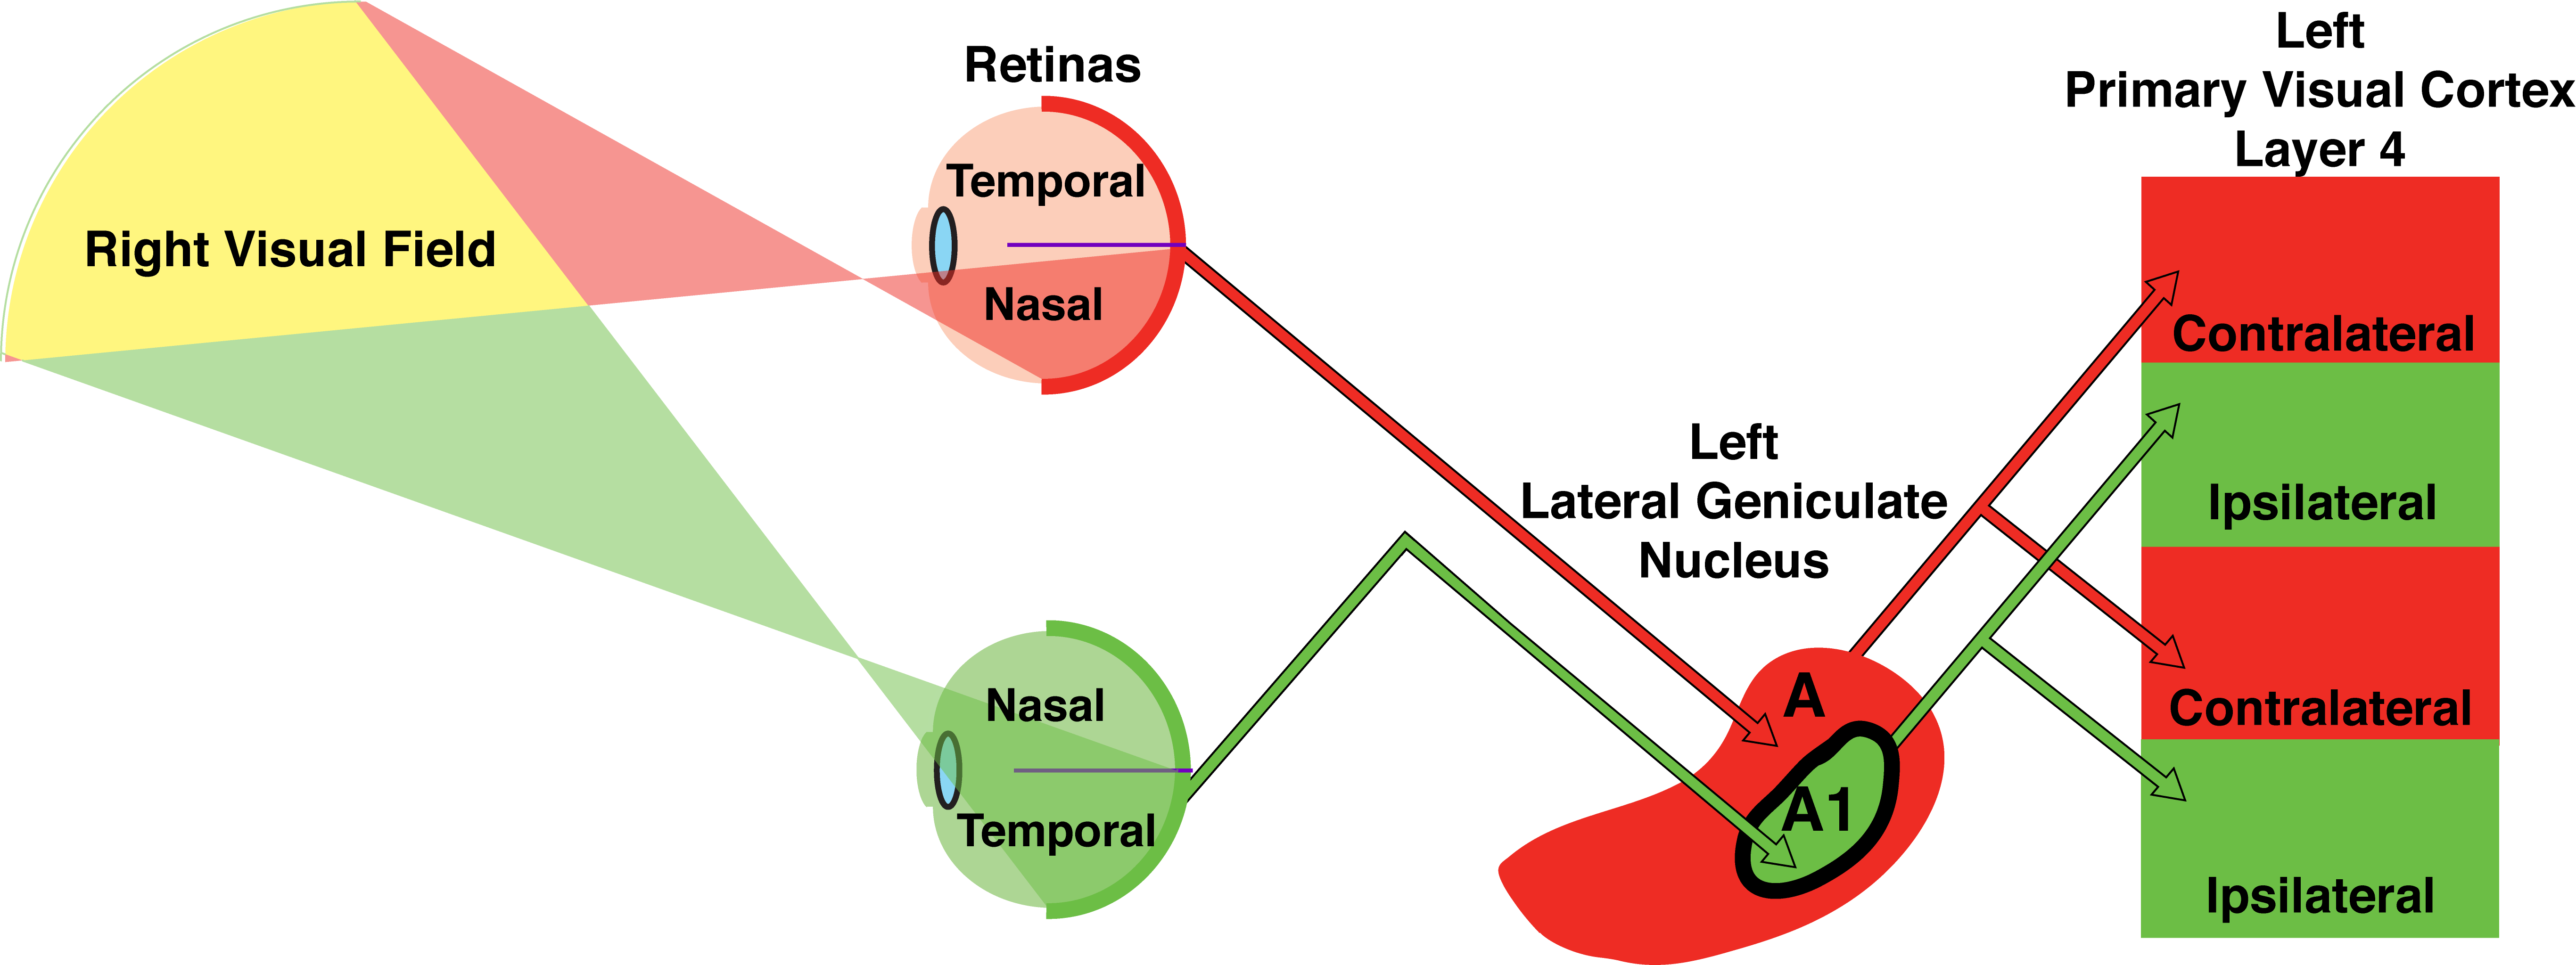
\includegraphics[width=1.0\textwidth]{FigureImages/visSystem.png}
\end{center}
\caption[Organization of the ferret visual system]{Organization of the ferret visual system.  The Left side of the visual system is depicted.  The right visual field is encoded by the right nasal retina and the left temporal retina.  Retinogeniculate afferents from nasal RGCs in the right retina cross the optic chiasm and terminate in the A lamina of the left LGN.  Afferents from temporal RGCs in the left retina do not cross the optic chiasm and terminate in the A1 lamina of the LGN.  Geniculocortical projections from the A and A1 laminae in the LGN then project to layer 4 of the primary visual cortex (V1).  These projections are segregated into non-overlapping patches of cells that respond preferentially to stimuli from either the ipsilateral or contralateral eye depending on the origin of their geniculocortical input. These segregated patches are the anatomical basis for ocular dominance.}
\end{figure}  
RGC axons exit the eye at the optic nerve head and proceed to the optic chiasm.  Axons from nasal RGCs cross the optic chiasm en route to the contralateral LGN and axons from temporal RGCs remain uncrossed en route to the ipsilateral LGN.  
	The ferret LGN is composed of two major retinorecipient laminae, A and A1.  There are also three minor retinorecipient layers in the lateral aspect of the nucleus known as C, C1, and C2.  They are omitted from the main discussion here as my focus on the LGN is largely about gross structural details. Lamina A receives input from the contralateral eye and lamina A1 receives input from the ipsilateral eye.  In the ferret, as well as in many higher mammals, the boundaries between these major anatomical divisions in the LGN are cell sparse interlaminar zones (Linden et al., 1981b).  Additionally, sublaminar divisions in the ferret LGN between the input of ON and OFF center RGCs to the A and A1 lamina are apparent (see section 1.1.2).  The ON/OFF sublaminar boundaries are also characterized by a lower density of cell bodies although not as dramatically as the interlaminar zones between the A and A1 laminae (figure 1.2).
\begin{figure}[htb]
\begin{center}
\leavevmode
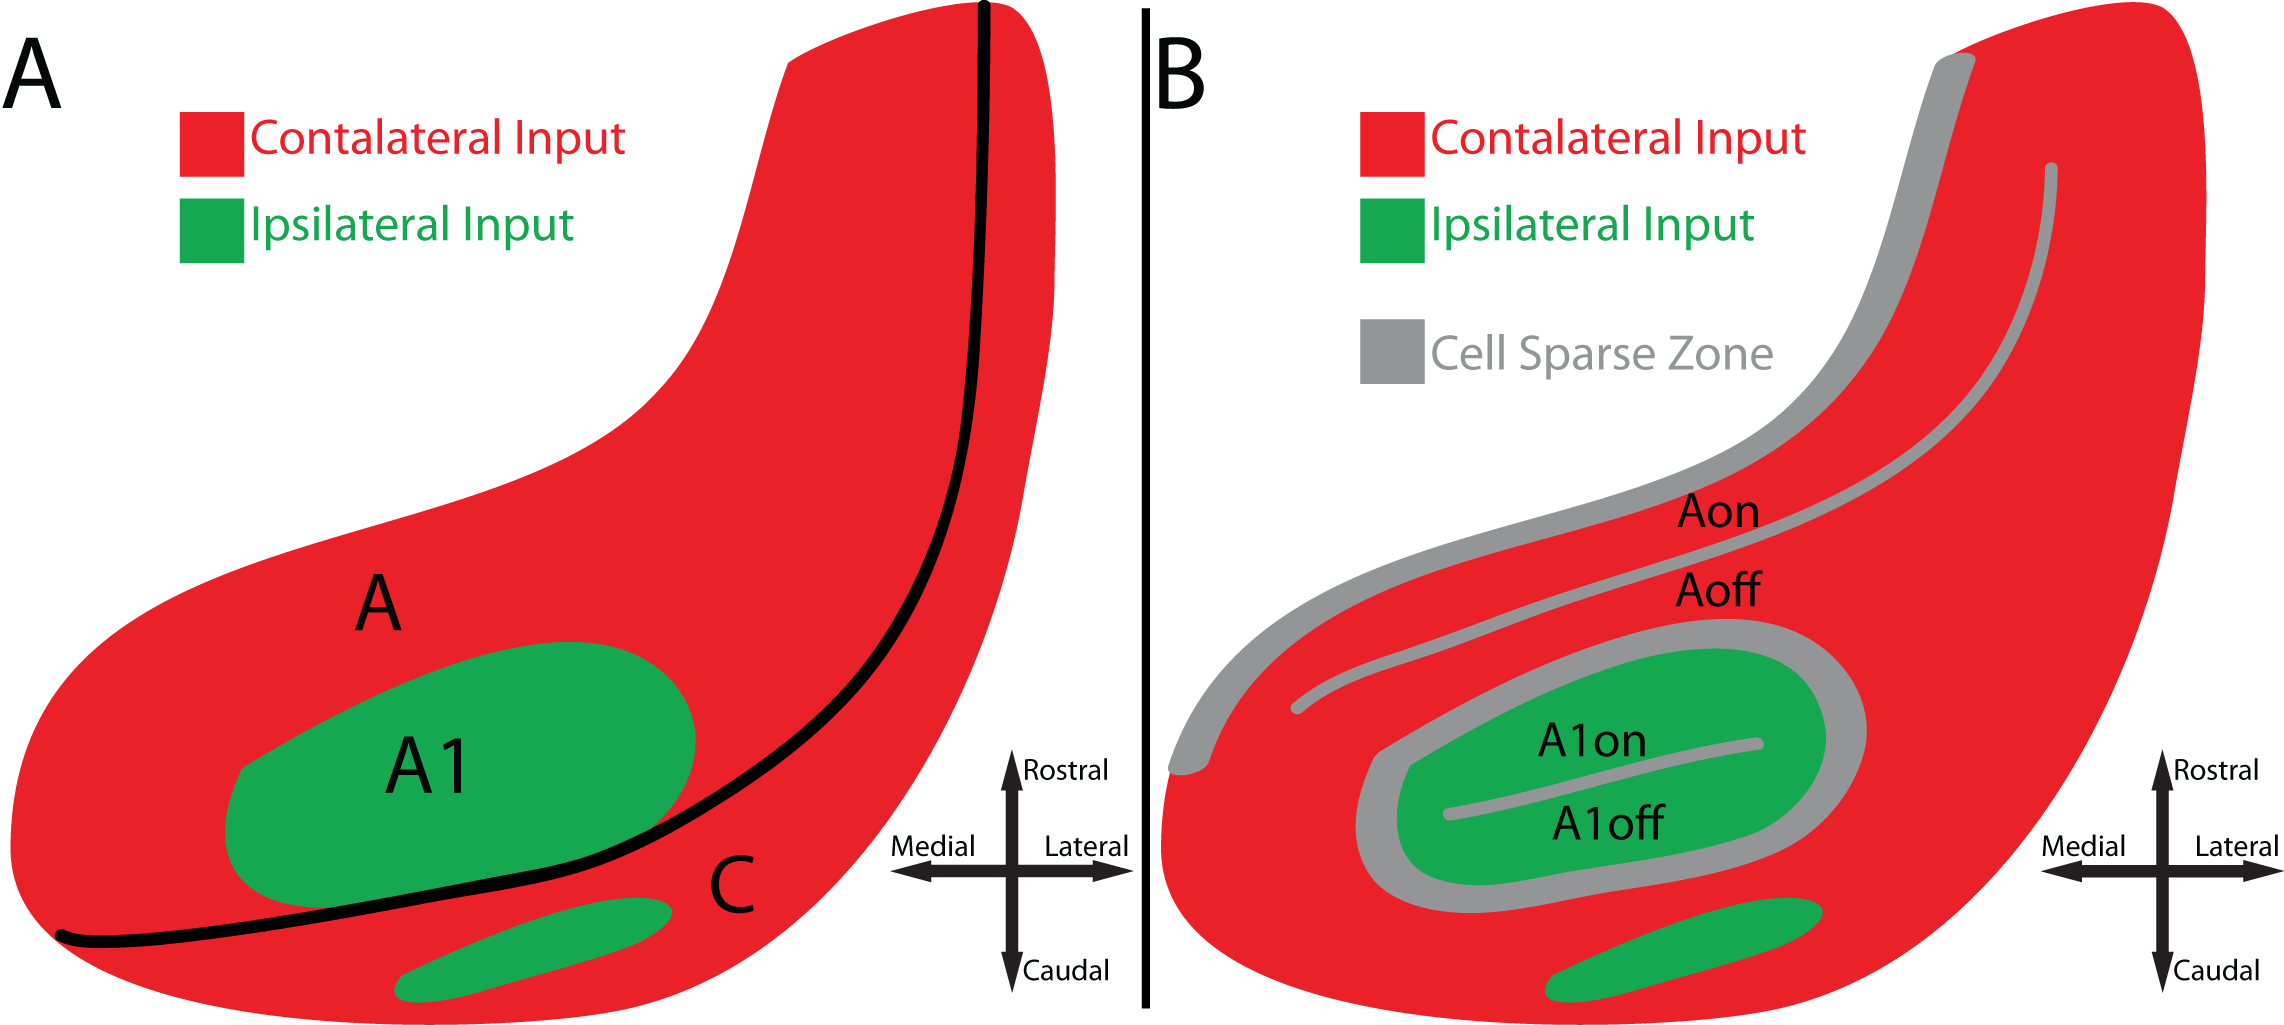
\includegraphics[width=1.0\textwidth]{FigureImages/NormalLGNLayers.png}
\end{center}
\caption[Laminar boundaries and sub-laminar divisions in the ferret LGN]{Laminar boundaries and sub-laminar divisions in the ferret LGN.  Both eyes send input via RGCs into the ferret lateral geniculate nucleus (LGN).  Contralateral input to the retina is shown in red and ipsilateral input to lamina A1 is shown in green.  A, major divisions of the LGN.  The LGN is composed of two major retinorecipient layers, the contralateral A layer and the ipsilateral A1 layer, as well as minor retinorecipient layers collectively depicted here as the C layer.  B, laminar boundaries and sublaminar divisions.  The medial boundary of the LGN, The A/A1 laminar boundary, and the A1/C laminar boundary are major cell sparse zones. Minor cell sparse zones delineate sub-laminar ON/OFF boundaries within the A and A1 layers.}
\end{figure}
	Geniculocortical projections from the A and A1 laminae of the retina terminate in layer 4 of primary visual cortex (V1). Geniculocortical projections in to layer 4 of V1 form non-overlapping projections representing contralateral and ipsilateral input from the  LGN from lamina A and A1, respectively.  As with other binocular mammals, this projection pattern forms the anatomical basis for ocular dominance (Hubel and Wiesel, 1962; Hubel and Wiesel, 1969; Hubel and Wiesel, 1972; Hubel and Wiesel, 1998).  However, this is not universally the case as rodents lack ocular dominance columns and some new world monkeys show a complete lack of or variable appearance of ocular dominance columns.  Additionally, rodents show ocular dominance at a cellular level.  The ferret visual system shows classic anatomically and physiologically defined ocular dominance as demonstrated in the cat and macaque and as such the insight gained from these models is applicable here.

\subsection{Physiology}
In the retina, visually driven responses of RGCs can be separated into two classes, ON and OFF.  For all RGCs, the receptive field is circular and is composed of center and surround.  ON RGCs respond well to a light presented in the center of their receptive field and decrease in response magnitude when a light is presented in their surround.  OFF RGCs respond in the opposite fashion; light presented to their receptive field$'$s surround increases their response, light presented to their receptive field$'$s center decreases their response.  In the ferret LGN, the same receptive field properties are maintained in geniculate relay neurons.  Responses driven through ON and OFF RGC input to the LGN are organized into ON and OFF sublaminar regions in both the A and A1 laminae (Figure 1.2 and Section 1.1.1)(Stryker and Zahs, 1983).  LGN cells responding to ipsilateral and contralateral inputs are also segregated in the LGN lamina (see Section 1.1.1).
	In layer IV of the primary visual cortex, receptive fields of neurons receiving direct input from the LGN become elongated in form are optimally driven by stimuli that are linear and oriented at a specific angle (Hubel and Wiesel, 1962). These receptive fields are the product of convergence by collinear LGN receptive fields onto a target layer IV neuron (Chapman et al., 1991).  Additionally, layer IV cells in primary visual cortex begin to integrate synaptic input from from both ipsilateral and contralateral inputs.  This integration leads to physiologically defined ocular dominance in which some cells respond preferentially to ipsilateral stimuli, some to contralateral stimuli, and some to both.  Depending on the species of binocular mammal, the ratio of cells driven by stimulation of ipsilateral, contralateral, or both eyes varies.  In many large binocular mammals, groups of cells sharing similar eye-specificity are arranged in periodic and interdigitated columns oriented orthogonal to the pial surface (Figure 1.3).  Physiological grouping of cells in this manner is observed as a result of segregated, eye specific, and spatially periodic input to the cortex from LGN thalamocortical projections (see Section 1.1.1).
\begin{figure}[ht!]
\begin{center}
\leavevmode
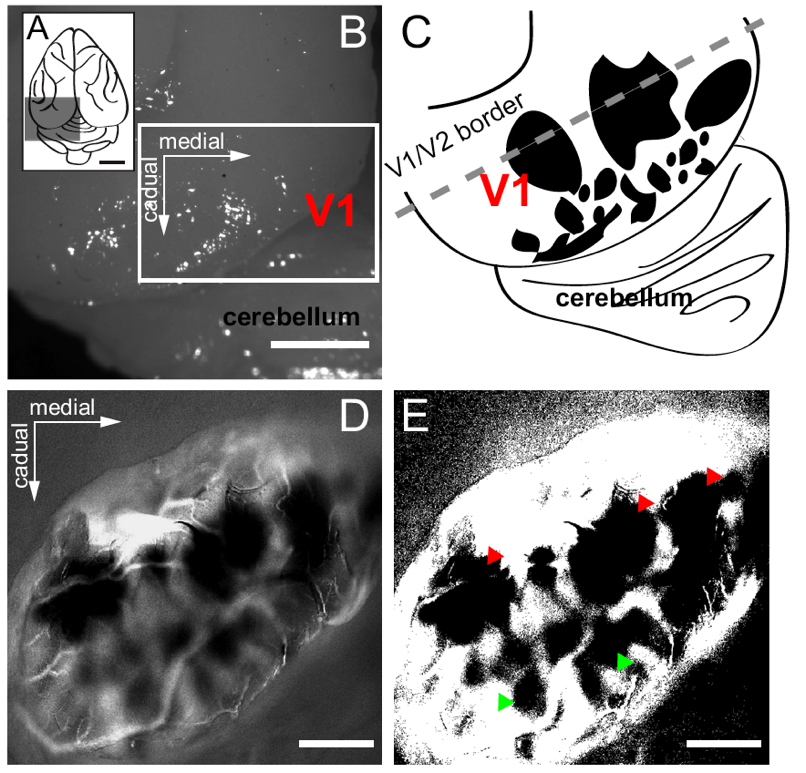
\includegraphics[width=0.8\textwidth]{FigureImages/ODCMap.png}
\end{center}
\caption[The ocular dominance column map in ferret V1]{The ocular dominance column map in ferret V1.  (A-B) Dorsal surface of the ferret cortex (A) Illustration of the ferret cortex with the caudal pole highlighted. (B) V1 is located on the dorsal ridge of the caudal most part of the ferret$'$s cortex. Scale bar=0.2 cm. (C) An illustration of the map of ocular dominance in the ferret with projections from one eye represented in black and the V1/V2 border represented as a gray line. (D) Intrinsic signal optical image of eye specific responses in V1. Black patches correspond to responses from one eye while lighter patches correspond to responses from the other eye. Scale bar = 1mm.  (E) Thresholded image of (B1) illustrates the unique organizational pattern of the ocular dominance column map in the ferret. Large blobs are located at the V1/V2 border (red arrows) and smaller columns are located at caudal pole (green arrows). Scale bar = 1 mm.  Figure courtesy of K. Padmanabhan.}
\end{figure}


\subsection{Visual Cortical Columns}
The visual cortex represents many features of visual stimuli using columnar systems.  The entire collection of a columnar system for a particular stimulus feature is referred to as a map of that feature (see Figure 1.3 for an example of one such map).  some of these maps such as the map of retinotopy vary continuously across the cortex  (Van Essen et al., 1984), while others such as ocular dominance are spatially periodic (Hubel and Wiesel, 1968).  Other classes of maps such as that of orientation are both periodic (single orientations are separated by others in the map) and continuous (the progression from one orientation through all other back to the original is smoothly mapped)(Hubel and Wiesel, 1974; Bonhoeffer and Grinvald, 1991).  Maps in both V1 and secondary visual cortex (V2) share these basic properties.  Ocular dominance columns are a feature of the visual system of many higher mammals.  Rodents show ocular dominance at the cellular level, but they lack the columnar organization seen in animals such as the macaque, cat and ferret.  Instead, the visual system of rodents is organized into a binocular response zone inside of a larger contralateral response zone (Hubener, 2003).  Single unit recording studies in higher mammals have shown that cells in V1 are arranged into spatially periodic ocular dominance columns in higher mammals (Hubel and Wiesel, 1962; Hubel and Wiesel, 1977).  The size of ODCs varies roughly with the size of the animal in which they are studied.  Ferret ODCs are on the order of 200-400�m (Issa et al., 1999), where as macaque ODCs vary between 500-800�m (Hubel and Wiesel, 1969).   Within a given species, the statistics of ODC size can vary from individual to individual but genetically similar animals (litter-mates for example) tend to share similar ODC sizes and distributions (Kaschube et al., 2002; Kaschube et al., 2003).  Column size and shape were traditionally thought to be relatively stable throughout development, but recent evidence suggests that columns may change in their geometric properties throughout development (Kaschube et al., 2009).

\section{Visual Critical Period}
In neuronal systems, critical periods are epochs of development in which circuits are maximally sensitive to changes in the pattern of neuronal activity (Hubel and Wiesel, 1962, 1970; Hubel et al., 1977).  Changes in the activity pattern of circuits during the critical period leads to sculpting of the circuit.  In the visual system, there are two identifiable critical periods.  The first is the critical period for proper eye specific segregation and laminar targeting in the retinogeniculate circuit. In the ferret, this period extends from birth to P25 and corresponds roughly to the period of time in which the retina is known to exhibit spontaneous activity in the form of retinal waves (see section 1.3.1) (Penn et al., 1998b; Penn and Shatz, 1999; Stellwagen and Shatz, 2002).  The retinogeniculate critical takes place before eye opening and thus is driven by endogenous activity patterns.  Activity in the retina during this developmental epoch can be thought of as instructing the proper segregation and laminar targeting of RGCs in the LGN (Huberman et al., 2008).  This idea is important for the work that I present in chapter 4 because I employ an established method for manipulation of retinal activity from P0-P10 in order to alter the normal projection and lamination patterns of RGC afferents in the LGN (Huberman et al., 2002).
The second critical period in the visual system is the geniculocortical critical period for ocular dominance plasticity in which the response of neurons in V1 can be shaped by the modification of external stimuli.  The geniculocortical critical period for ocular dominance plasticity in the ferret begins at P35 and ends at P70-80 (Issa et al., 1999).  Unlike the retinogeniculate critical period, the geniculocortical critical period for ocular dominance plasticity occurs after eye opening.  Importantly, this means that the major source of activity in the system during this developmental phases is non-endogenous and that the geniculocortical critical period occurs after the initial formation of ocular dominance columns (Hubel and Wiesel, 1962; Hubel and Wiesel, 1963; Issa et al., 1999; Crowley and Katz, 2000).  This critical period can thus be thought of as a period of time in which the visual system is capable of sculpting its existing architecture to fit the constraints placed upon it by the specific anatomy of the animal and the environment in which the animal lives.  Deprivation of one eye from external stimulation during this critical period results in a shift of responses in V1 neurons toward the non-deprived eye as well as a reduction in the size of deprived eye ocular dominance columns.  This process is mediated by a retraction of geniculocortical axons from the deprived eye and an elaboration of those from the non-deprived eye (Hubel et al., 1977; LeVay et al., 1980).  Geniculocortical critical periods for ocular dominance plasticity have been identified in many mammalian species including the cat (Wiesel and Hubel, 1963; Hubel and Wiesel, 1970), primate (Hubel et al., 1977; Horton and Hocking, 1997), and the ferret (Issa et al., 1999).  The opening at of this critical period in the ferret at P35 directly follows eye opening at P30-35.  In the work presented here, I perform the imaging experiments described in chapter 2 during the geniculocortical critical period in an attempt to characterize the molecular profile of visual cortex during this developmentally relevant epoch. 

\section{Spontaneous Activity in the Visual System}
Spontaneous activity during the development of the visual system is observed at the level of the retina, the LGN and V1.  All of these sources of spontaneous activity occur at different points during development, but they all occur before the onset of externally driven activity in the system and are correlated with the maturation of normal anatomy throughout the system (figure 1.4).  In all discussion below, the timing of spontaneous activity is reported for the ferret.
\begin{figure}[htb]
\begin{center}
\leavevmode
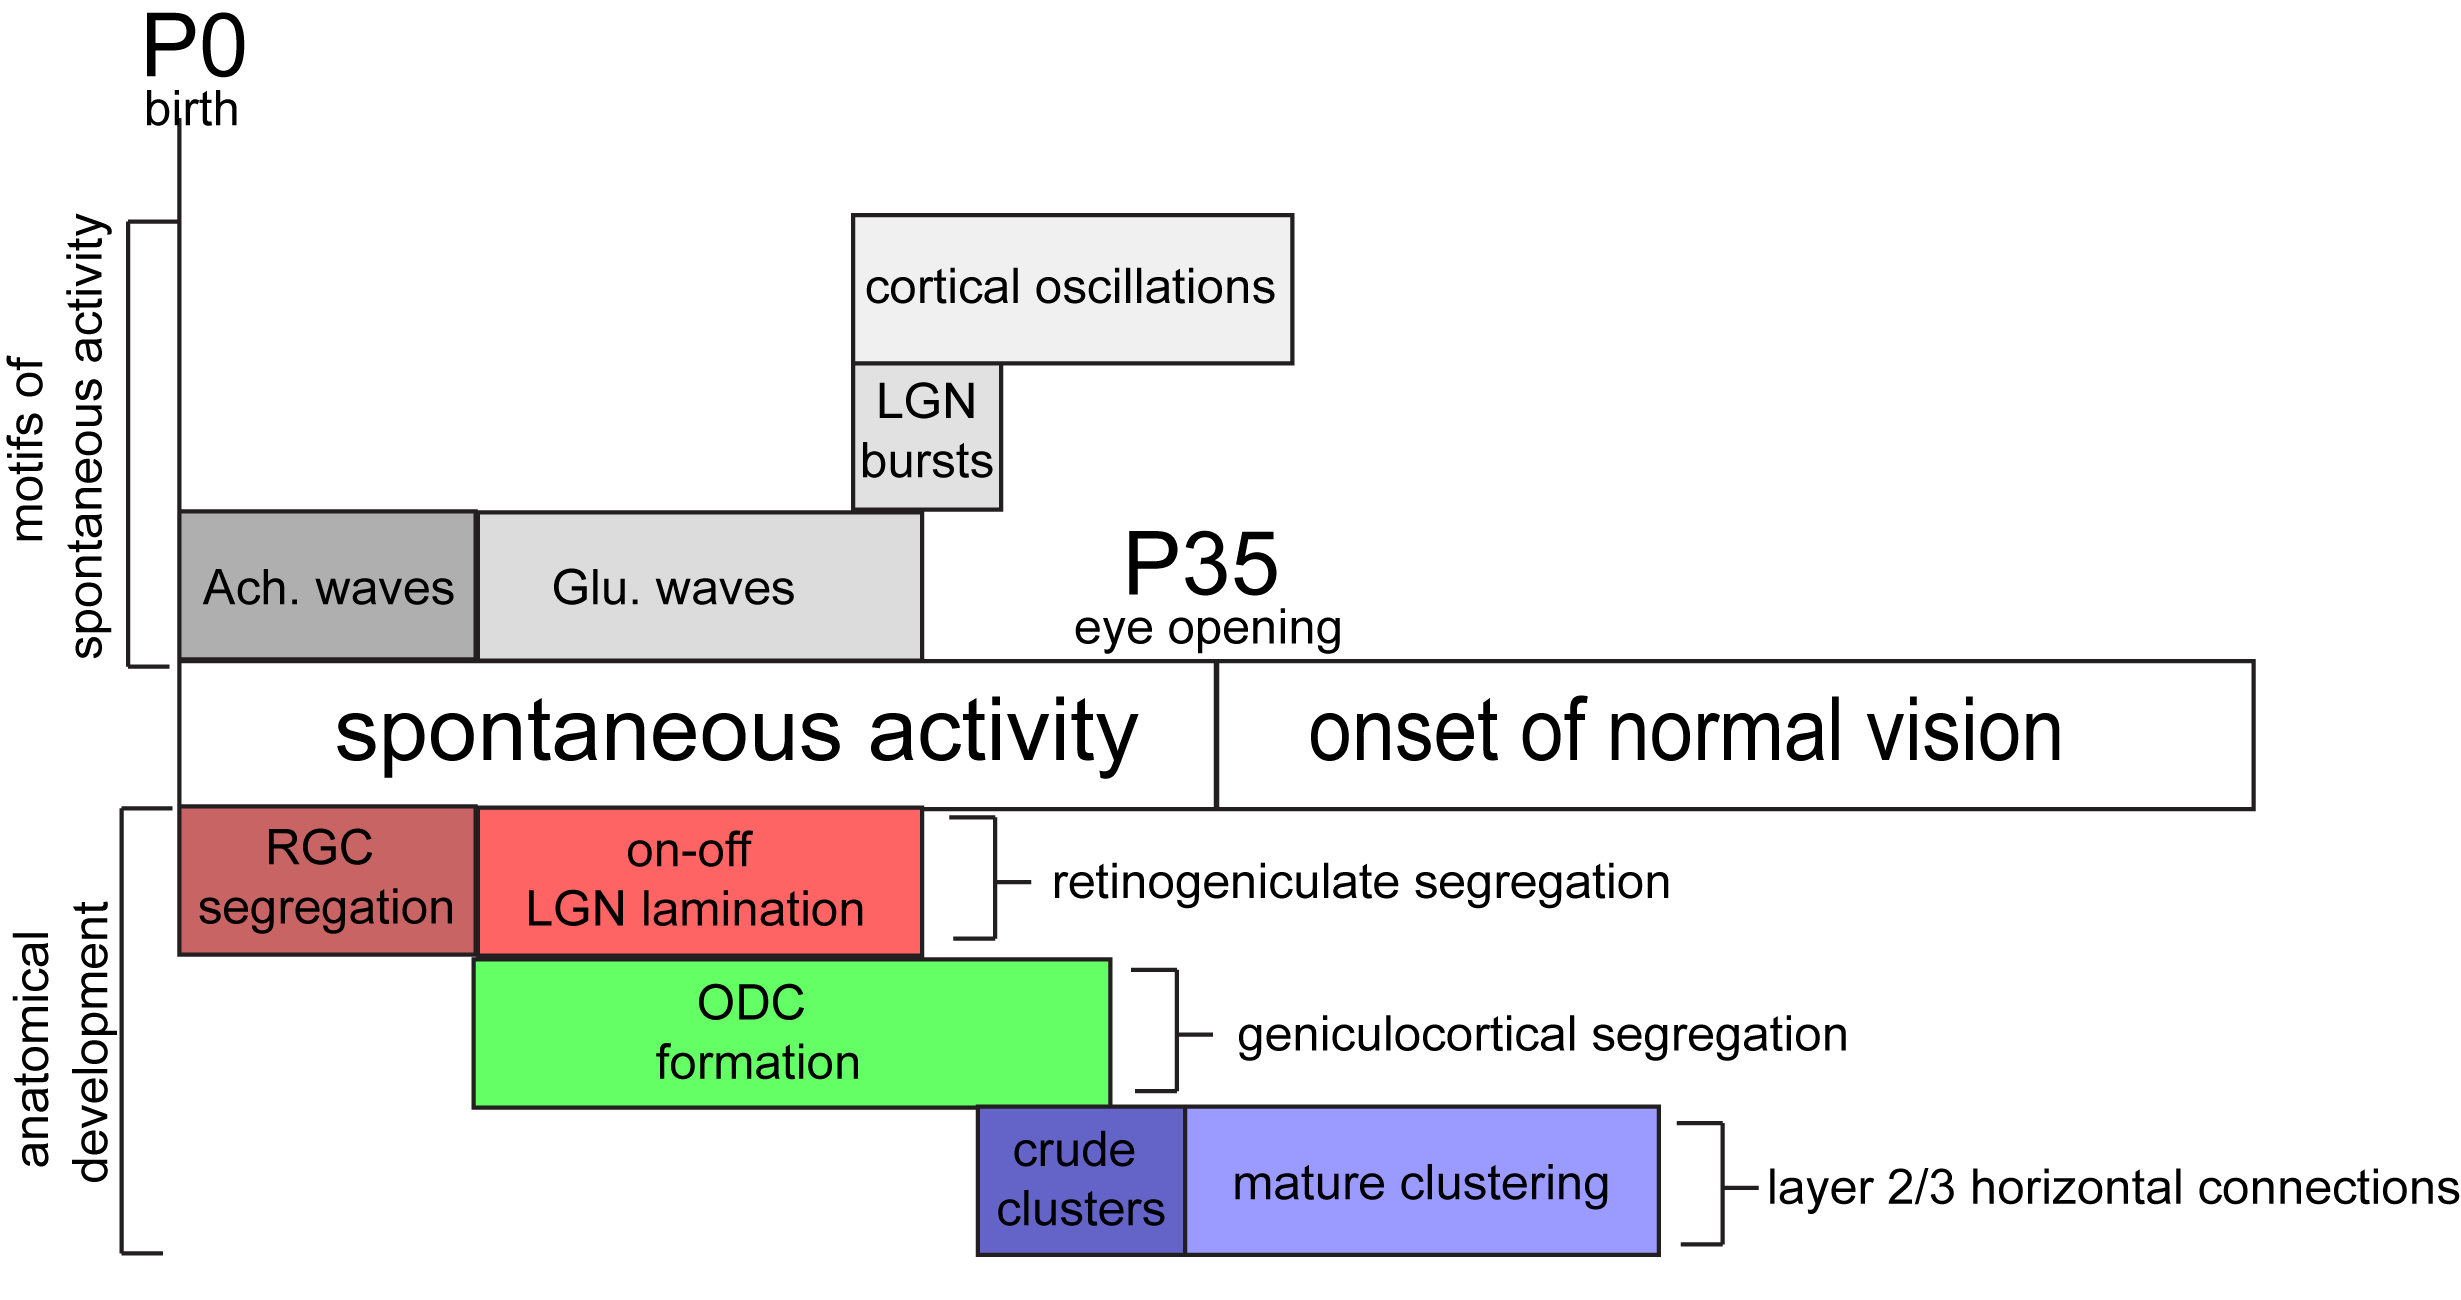
\includegraphics[width=1.0\textwidth]{FigureImages/spontaneousActivityTimeline.png}
\end{center}
\caption[Illustration of anatomical development in the ferret visual system and concordant patterns of spontaneous activity]{Illustration of anatomical development in the ferret visual system and concordant patterns of spontaneous activity.  (Adapted from Issa, Trachtenberg, et al 1999).  Timeline begins at P0 with birth.  Between P0 and P25, retinal waves dominate as the principle type of spontaneous activity (reviewed by, Wong 1999, Huberman, Feller, et al, 2008).  In the third postnatal week of life LGN bursts have been identified (Weliky and Katz, 1999).  During the same time, cortical oscillations have been recorded (Chiu and Weliky, 2002).  During the period of spontaneous activity, the retinogeniculate circuit (red), the geniculocortical circuit (green) and the corticocortical connections (blue) in V1 are undergoing maturation. Figure courtesy of K. Padmanabhan.}
\end{figure}

\subsection{Retinal Waves}
At birth, endogenous activity in the retina takes the form of traveling waves of cholinergic activity initiated in starburst amacrine cells (Feller et al., 1996; Penn et al., 1998b; Feller, 1999). This pattern of activity persists in the retina for the first two weeks of postnatal life (figure 1.4).  These traveling waves are composed of bursting patterns that last from 1 to 8 seconds and occur from 30 to 60 times per hour (Wong et al., 1993).  cholinergic retinal waves appear to be involved in the proper segregation of and laminar targeting of eye specific inputs into the LGN.  Disrupting these waves dramatically impacts both the initial and final projection scheme of the RGC afferents in the LGN (Huberman et al., 2002)   During the second week of postnatal life, a second kind of retinal wave is observed.  The second class of retinal wave are mediated by glutamate transmission, begin at P10, and last at least as long as P25 (Wong and Oakley, 1996; Stacy and Wong, 2003; Kerschensteiner and Wong, 2008).  Glutamate mediated retinal waves manifest themselves differently across the ON and OFF populations of RGCs.  The ON RGCs are relatively less active than the OFF centered cells as measured by burst frequency.  The ON cells fire ~50 burst per hour where the OFF cells may reach activity levels of up to 250 bursts per hour (Wong and Oakley, 1996; Kerschensteiner and Wong, 2008).  Glutamate mediated retinal waves are necessary for both the maintenance of eye specific segregation and the formation of ON/OFF sublaminar boundaries in the LGN.

\subsection{Spontaneous Activity in the LGN}
Prior to eye opening in the ferret, the LGN exhibits spontaneous activity in the form of bursting activity that propagate across the nucleus (figure 1.4).  These waves of activity, known as spindle waves, tend to propagate from the along the dorsal ventral axis of the nucleus (Bal et al., 1995; Kim et al., 1995; McCormick et al., 1995).  Spindle waves in the LGN are well correlated within laminae (A, A1, C), but not across laminae (Weliky and Katz, 1999).  Retinal and cortical inputs to the LGN appear to play a large role in shaping LGN bursting activity prior to eye opening.  When the eyes are removed, the LGN continues to burst but there is a much lower correlation within each lamina in the bursting pattern observed (Weliky and Katz, 1999).  If V1 is removed, the bursting activity in the LGN stops entirely, suggesting that the geniculocortical and corticogeniculate circuits are required for the maintenance of LGN bursting (Weliky and Katz, 1999).  The loss of LGN bursting in the absence of V1 is most likely due to both severing of geniculocortical afferents and the loss of corticogeniculate feedback to the LGN (Blumenfeld and McCormick, 2000).  LGN bursting appears to have an influence on the development of geniculocortical projections in V1.  When the LGN is prevented from bursting using an infusion of TTX for activity block in the kitten, The spatial spread of individual LGN afferents in V1 is greater.  This increased projection is either a spread in the normal projection or a failure to prune aberrant connections (Catalano and Shatz, 1998).

\subsection{Spontaneous Activity in V1}
In V1, spontaneous activity takes the form of oscillations that are distributed across the cortical sheet from ~P24 to P29 (figure 1.4).  These oscillations appear to be most well correlated across spatial scales of around 800�m, suggesting a relationship with the geometry of ocular dominance columns.  In fact, there is a high correlation of spontaneous activity between sites in the cortex with the same ocular preference (Chiu and Weliky, 2001).  However, the periodic pattern cannot be completely explained by a correlation with the underlying geometry of ocular dominance columns.  The correlation of spontaneous activity across V1 is instead better thought of as a function of both ocular dominance and orientation preference (Chiu and Weliky, 2001; Chiu and Weliky, 2002).  
The degree to which spontaneous activity in V1 may be shaping the anatomy of V1 connections is unclear.  It is unlikely that spontaneous activity instructs the formation of ocular dominance columns because geniculocortical afferents are already in place before the onset of spontaneous activity in V1 (Crowley and Katz, 2000).  However, the development of orientation preference may be a different story.  It is thought that orientation preference is shaped by the development of horizontal projections in layer 2/3 (Ruthazer and Stryker, 1996; Bosking et al., 1997).  At the onset of spontaneous activity in V1, layer 2/3 neurons are migrating into place and the structure of horizontal connections between different locations in layer 2/3 are crude at best (Jackson et al., 1989; Ruthazer and Stryker, 1996).  It is therefore possible that spontaneous activity in V1 serves to guide the development of orientation tuning and layer 2/3 horizontal projections before the onset of vision.

\section{The Retinogeniculate Circuit}
\subsection{Structure of the Retinogeniculate Circuit}
The projection pattern of RGCs into the LGN define the different lamina in the LGN.  The major projection into the LGN from the contralateral eye defines the A lamina, the major projection of the ipsilateral eye defines the A1 layer, and the minor projections of the eyes define the C0, C1, and C2 layers (Linden et al., 1981a)(figure 1.2).  The A and A1 laminae are further divided into ON and OFF sublaminar regions into which ON and OFF center RGCs project, respectively.

\subsection{Development of the Retinogeniculate Circuit}
The stereotyped morphology of the retinogeniculate circuit is not present and early stages of visual development.  The final structure of the circuit is instead gradually refined during early development (Huberman et al., 2008).  In the ferret, initial projections into the LGN arrive from the contralateral retina and diffusely spread throughout the nucleus.  Shortly after contralateral projections arrive, projections from the ipsilateral retina innervate the nucleus and also spread over a large portion of the nucleus.  The resulting pattern is one of heavy overlap between the contralateral and ipsilateral projections into the nucleus at birth.  Over the course of the next ten days, the projections of the two eyes selectively prune back into their final eye specific laminae (Linden et al., 1981b; Cucchiaro and Guillery, 1984)(figure 1.5a).  During the first period of overlap, the afferents from the two eyes form functional synapses which are capable of driving LGN activity of cells located in the both nascent A and A1 laminae (Shatz and Kirkwood, 1984).  Inappropriate synapses are  eliminated though a competition dependent process.  Eliminating competition between the two eyes through either binocular enucleation or treatment with TTX results in a mature nucleus that lacks segregation of retinal inputs.  (Sretavan and Shatz, 1986; Shatz and Stryker, 1988).  
During the same developmental epoch, the cytoarchitecture of the mature LGN is beginning to develop.  At birth, the cell sparse interlaminar zones that are the hallmark of LGN laminae in the adult nucleus are not present.  Over the course of the first two postnatal weeks, cell sparse interlaminar zones begin to develop at the PGN/A, A/A1, and A1/C boundaries.  After the fourth postnatal week, the cell sparse interlaminar zones are in their adult form(Linden et al., 1981a).  Additionally, the A and A1 laminae are divided by minor cell sparse regions into ON and OFF leaflets (Stryker and Zahs, 1983; Zahs and Stryker, 1988; Cramer and Sur, 1997)(figure 1.5b).
\begin{figure}[ht!]
\begin{center}
\leavevmode
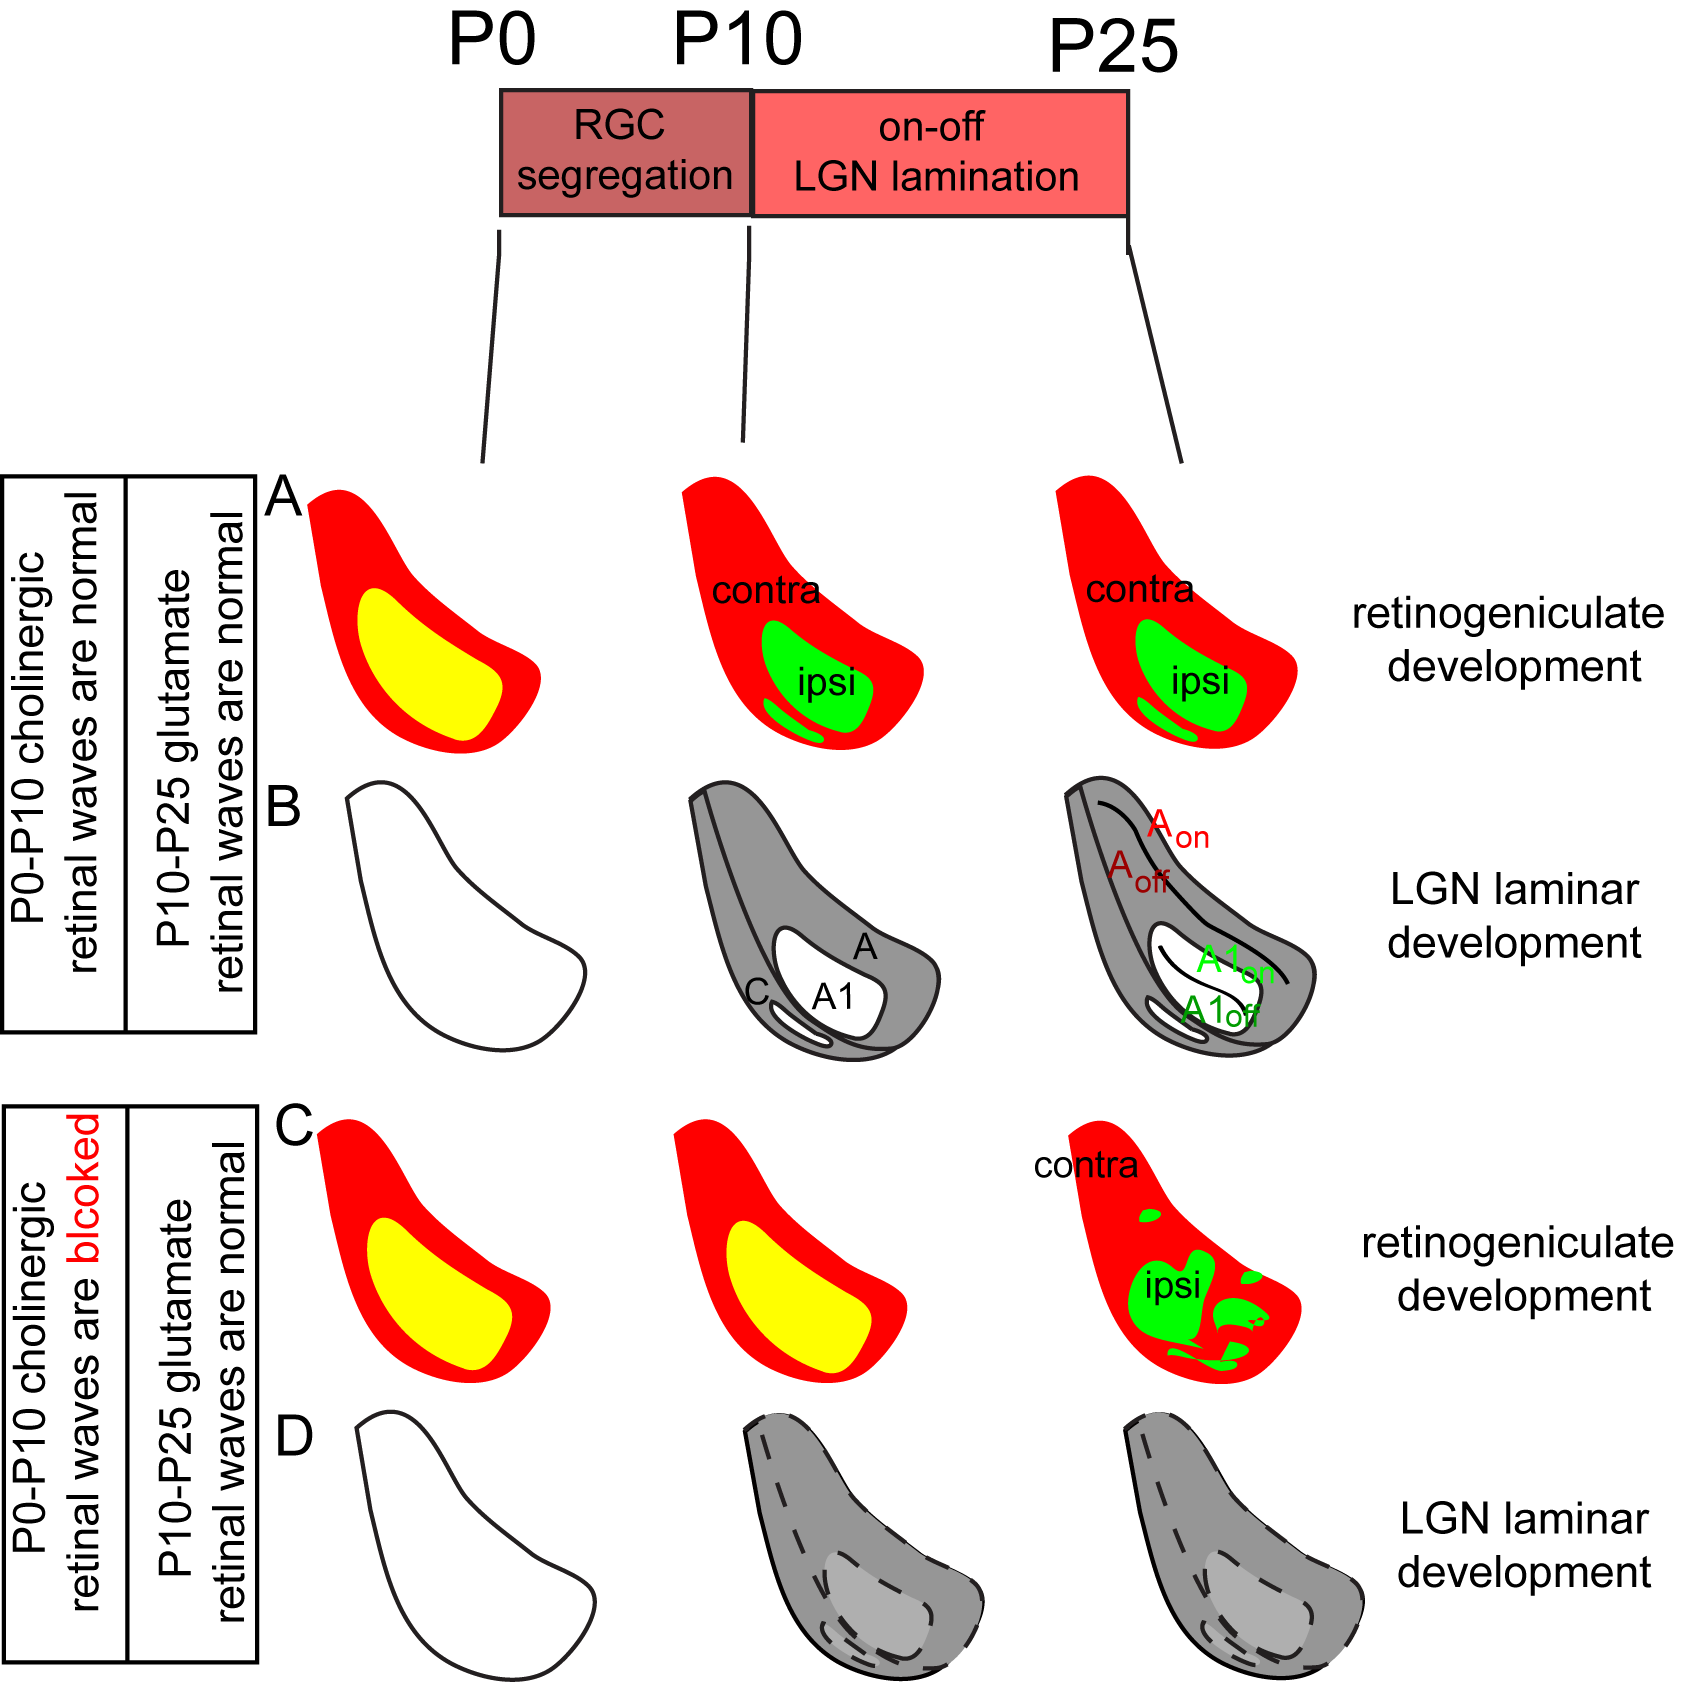
\includegraphics[width=0.8\textwidth]{FigureImages/LGNDevelopmentTimline.png}
\end{center}
\caption[Development of retinogeniculate projections]{Development of retinogeniculate projections.  Development of retinogeniculate projections (A) The developmental segregation of
retinogeniculate projections between P0 and P25. (B) Laminar maturation of the LGN between P0 and P25. (C) The developmental segregation of retinogeniculate projections between P0 and P25 when cholinergic retinal waves are blocked between P0 and P10 and glutamate waves are normal between P10 and P25. (D) Laminar maturation of the LGN between P0 and P25 when cholinergic retinal waves are blocked between P0 and P10 and glutamate waves are normal between P10 and P25.  Figure courtesy of K. Padmanabhan.}
\end{figure}

\subsection{The Role of Activity in Retinogeniculate Development}
The proper development of the retinogeniculate projection is dependent on the influence of endogenous retinal activity in the form of retinal waves (see section 1.3.1).  If cholinergic retinal waves are disrupted during the first ten days of life with either the cholinergic antagonist epibatidine (Penn et al., 1998a; Huberman et al., 2002; Huberman et al., 2003) or the sodium channel blocker TTX (Shatz and Stryker, 1988), the initial overlap of retinal projections observed at birth is preserved (figure 1.5c).  If only one of the eyes is subjected to disruption of retinal waves, segregation does occur. Unlike in the normal animal, the projection territory of the manipulated eye in both LGN is much reduced (Penn et al., 1998a).  This result frames the segregation of eye specific projections in the LGN as an activity dependent process.  Further evidence of implicating eye specific segregation as an activity dependent process is found when the activity of one eye is artificially increased through the application of the cAMP agonist forskolin.  When treated with forskolin, the projections of the treated eye expand relative to their normal territory (Stellwagen et al., 1999; Stellwagen and Shatz, 2002).  
Even though eye specific segregation is not observed at P10 after blockade of cholinergic retinal waves in the ferret, if the animal is allowed to recover until P25 (Huberman et al., 2002) or later (P30, see chapter 4), eye specific segregation does occur.  However, the normal pattern of projections is disrupted and normal LGN laminae do not develop (Huberman et al., 2002, chapter 4, figure 1.5c and d).  Under this scheme, cholinergic retinal waves are disrupted until P10, but glutamatergic retinal waves remain normal from P10 to P25.  Glutamatergic retinal waves are thus sufficient to drive eye specific segregation, but not normal formation of LGN laminae.  This observation allows the two processes to be studied independently if cholinergic retinal waves are disrupted until P10.  I make use of this manipulation in chapter 4 to characterize the relationship of a novel molecular marker for LGN development, collapsin response mediator protein 4 (CRMP4), to eye specific segregation and laminar development in the LGN.

\subsection{The Role of Molecular Cues in Retinogeniculate Development}
At the level of the optic chiasm, molecular cues play a large role in the proper targeting of retinal afferents to either the ipsilateral or contralateral LGN.  ventrotemporal RGCs normally project to the ipsilateral LGN and dorsomedial RGCs normally project to the contralateral LGN.  When deficient in key molecular cues, this normal projection scheme of retinal afferents is altered. Contralateral projecting RGCs normally express the transcription factor Islet-2 (Isl2), but when Isl2 expression is knocked out in the mouse, there is a significantly larger ipsilateral projection (Pak et al., 2004).  Conversely, defects in the expression of the transcription factor Zic2 or cell surface receptors such as EphBs  result in a significantly larger contralateral projection (Williams et al., 2003; Pak et al., 2004).  Additionally regulation of these markers occurs through the action of other transcription factors. Foxd1 expression is in the ventromedial retina and is linked to ipsilateral afferent targeting (Herrera et al., 2004).  Contralateral targeting programs are driven by the expression of Foxg1(Tian et al., 2008).  
Once in the LGN, the elaboration of retinal afferents into the appropriate topographic and eye specific target regions has also been shown to be under the control of molecular cues.  Targeting of RGC afferents is guided by matching the expression of various Eph cell surface receptors to gradients of the ligands, the Ephrins, in the LGN (Flanagan and Vanderhaeghen, 1998; Frisen et al., 1998; Huberman et al., 2005; Pfeiffenberger et al., 2005).  Additional guidance of topographic projection is driven by cues such as Ten-m3(Leamey et al., 2007).  Further evidence that retinogeniculate circuit patterning is subject to molecular influences comes from the study of the A2/A3/A5 triple knockout of the Ephrin A family in the mouse.  In this line, the mapping of visual space along the azimuth is completely abolished (Cang et al., 2005; Cang et al., 2008b; Cang et al., 2008a) and the pattern of eye specific projections resembles that of the LGN after blockade of cholinergic retinal waves.

\section{The Geniculocortical Circuit}
\subsection{Structure of the Geniculocortical Circuit}
In most mammalian species, geniculocortical afferents from eye specific laminae in the LGN terminate into layer 4 of the cortical sheet in a periodic fashion.  This periodic eriodic termination pattern of geniculocortical afferents into visual cortex is the anatomical basis of ocular dominance columns (Hubel and Wiesel, 1969; Hubel and Wiesel, 1972).  In the ferret, the organization of eye specific terminations into visual cortex form ocular dominance columns, but the organization of ocular dominance columns is unique among mammals (Redies et al., 1990; White et al., 1999b).  The termination pattern of geniculocortical afferents in the visual cortex of the ferret is composed of three distinct domains (figure 1.6).
\begin{figure}[ht!]
\begin{center}
\leavevmode
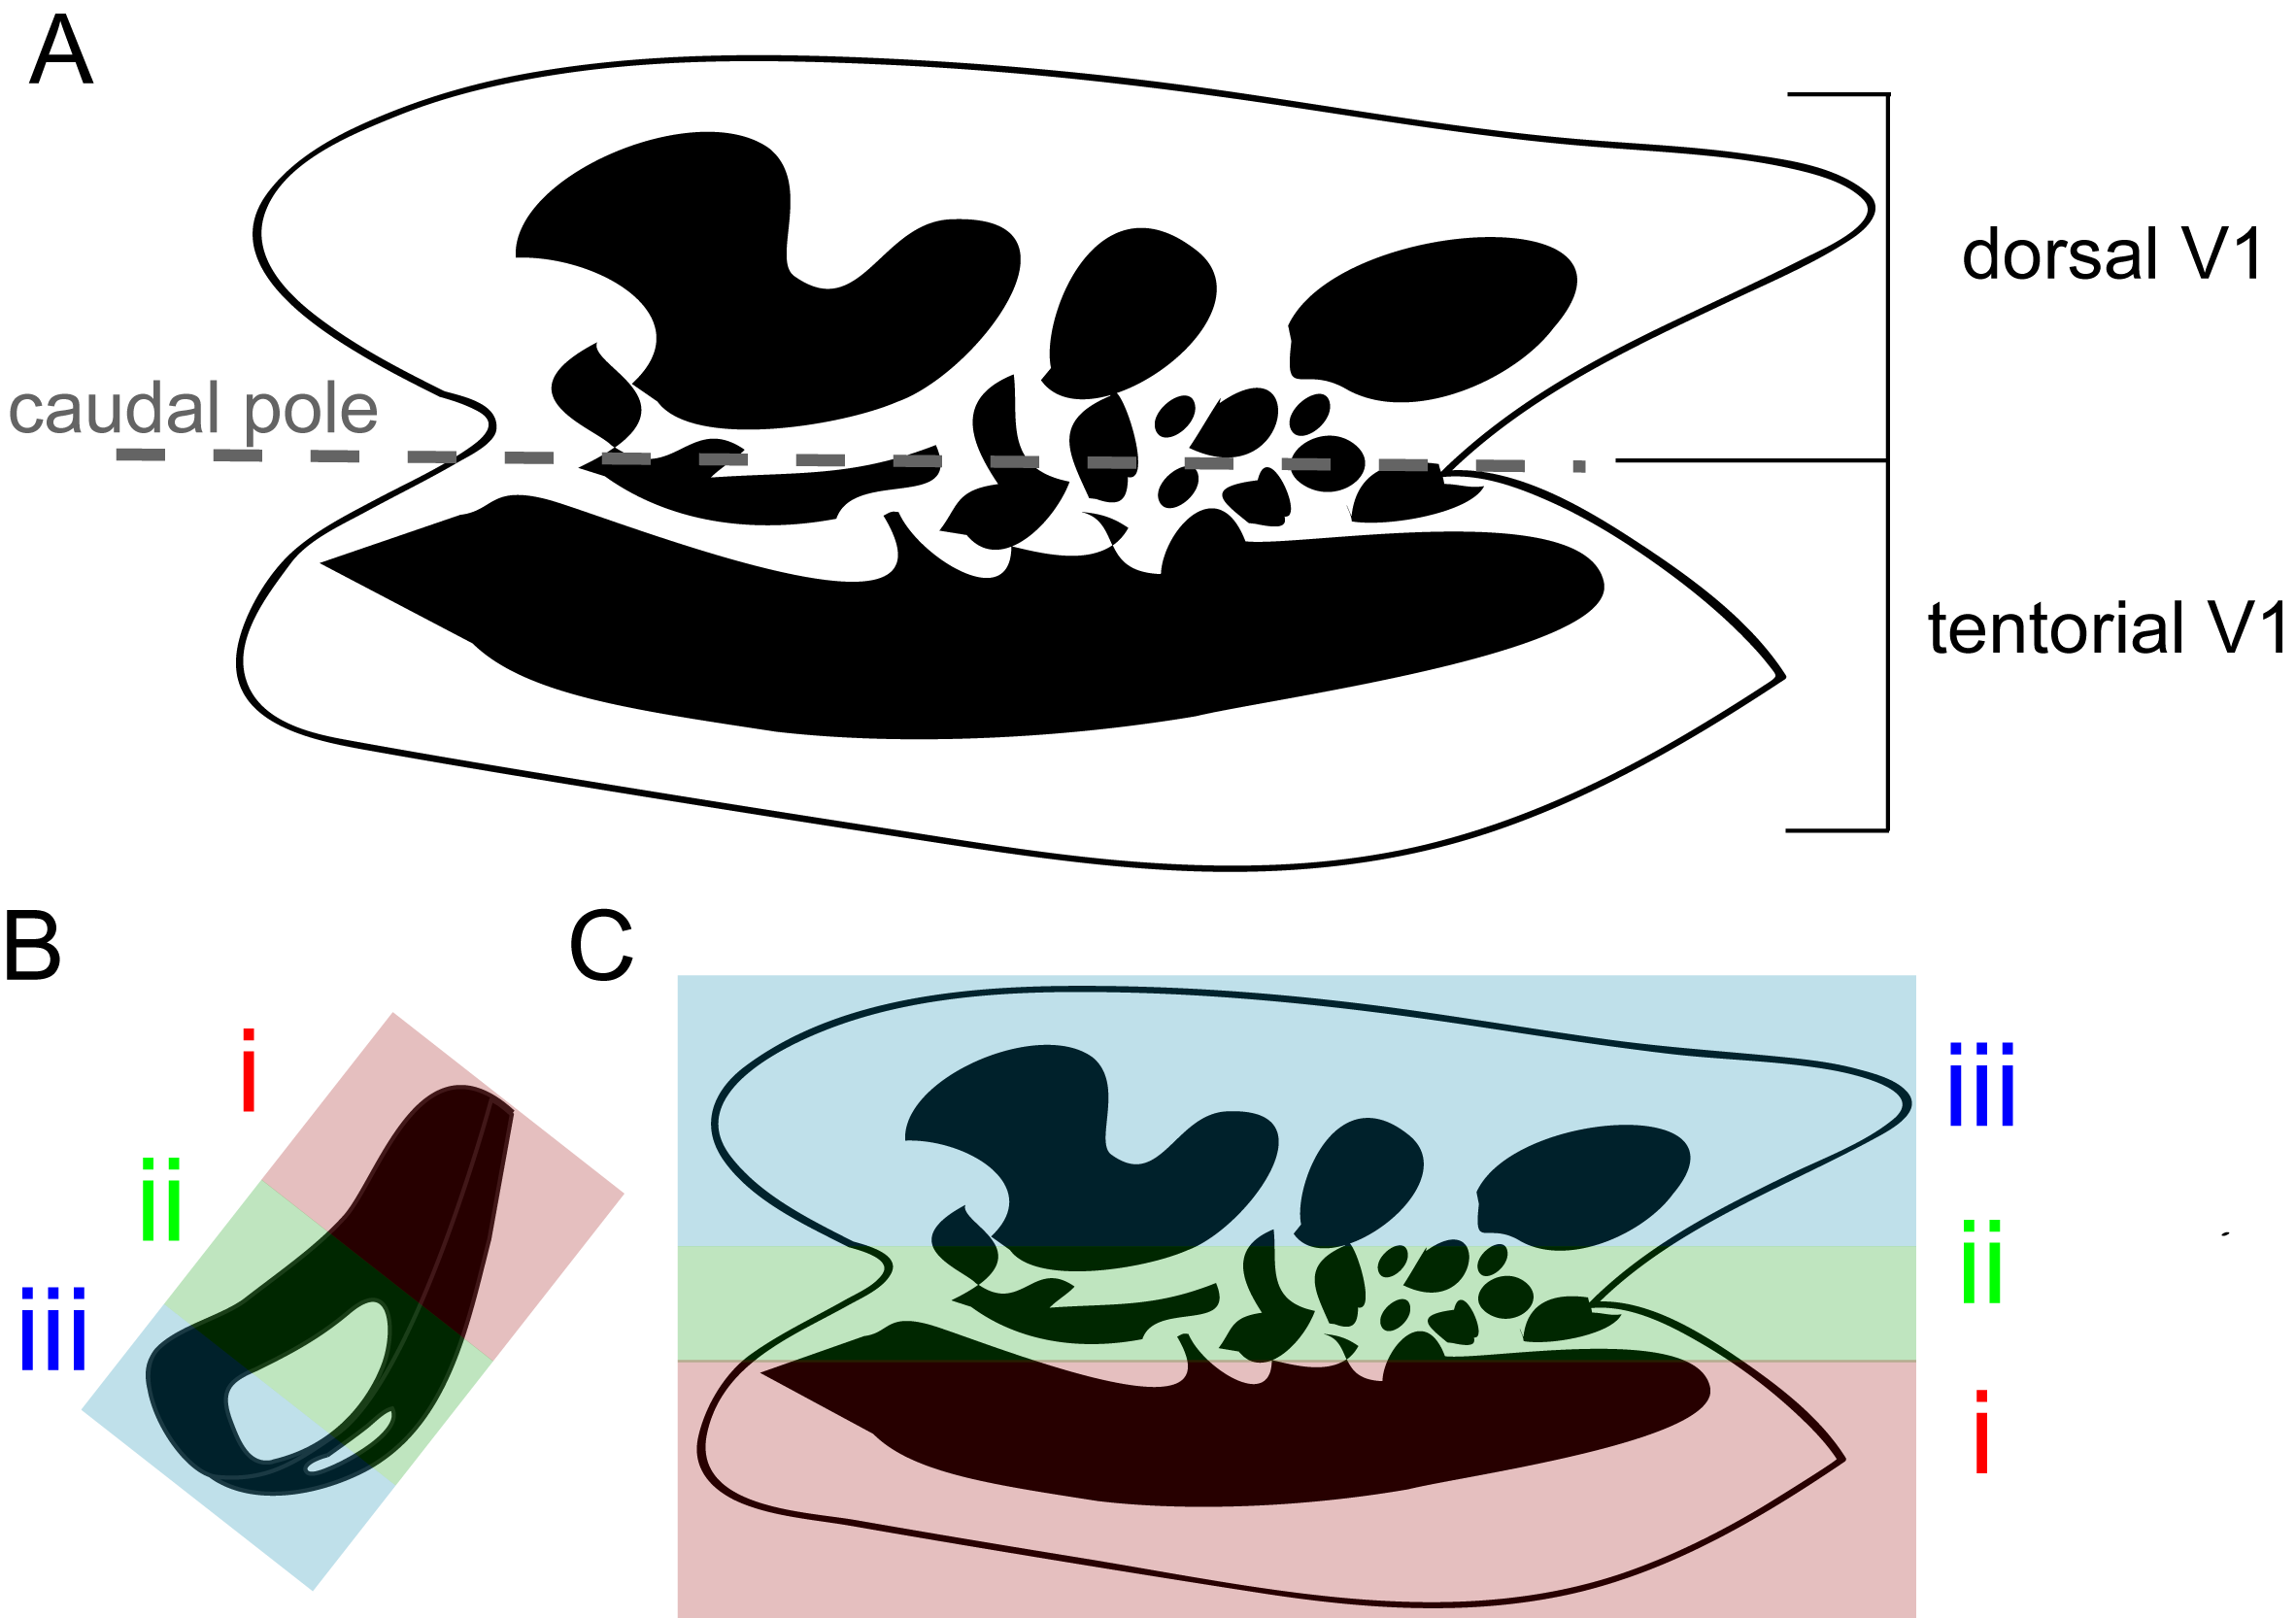
\includegraphics[width=0.8\textwidth]{FigureImages/ODCCartoon.png}
\end{center}
\caption[Schematic diagram of ferret V1]{Schematic diagram of ferret V1. (A) Schematic of a surface reconstruction of ferret V1 with the ocular dominance column termination pattern illustrated. The caudal pole is identified with a gray dashed line. The dorsal surface of V1 is composed of regular ocular dominance columns and the V1/V2 border columns. The tentorial (ventral part of cortex that begins at the caudal pole) surface is composed of regular ocular dominance columns and a continuous projection from the lamina A. Contralateral ocular dominance columns from lamina A are illustrated in black. The interleaving white domains correspond to ipsilateral ocular dominance columns from lamina A1. (B) Schematic of the LGN and the (C) cortex as in A. Three different regions of the LGN geniculocortical axons project to the three regions of V1. (red) Region i from the rostral lamina A in the LGN forms the geniculocortical projection to the continuous contralateral projection on the tentorial surface. (green) Region ii from the binocular LGN sends projections from both lamina A (black) and lamina A1 (white) to the tentorial surface and the dorsal surface of V1. (blue) Region iii from the binocular LGN sends projections from both lamina A (black) and lamina A1 (white) to the dorsal surface of V1 to form the large ocular dominance that compose the V1/V2 border.  Figure courtesy of K. Padmanabhan.}
\end{figure}
The first domain receives input from the most caudal binocular portion of the LGN and is the rostral most termination site of LGN afferents (blue area iii, figure 1.6).  Lamina A of the LGN innervates contralateral columns and lamina A1 of the LGN innervates ipsilateral columns.  This domain is composed of both V1 and V2 ocular dominance columns and columns here can be as large as 1mm.  The cytoarchitectural makeup of this area is homogenous and lacks defined boundaries between V1 and V2 as is observed in the cat and primates (Rockland, 1985; Law et al., 1988).  As a consequence, the only reliable way to define the V1/V2 border in the ferret is through physiological mapping of visual space (White et al., 1999, but also see section 2.3.3).
The second geniculocortical projection domain in the ferret visual cortex receives input from the central binocular portion of the LGN and is located at the caudal pole of  the visual cortex (green area ii, figure 1.6).  Similar to the first domain, contralateral columns are innervated by projections from lamina A of the LGN and ipsilateral columns are innervated by afferents from lamina A1.  Ocular dominance columns in this region are definitively part of V1 and are ~400�m in size.  These columns are similar in size and shape to those found in the cat. 
The third domain recieves input from the rosteral most portion of the LGN and is located on the tentorial (ventral) surface of the cortex after it has wrapped around the caudal pole (area i, figure 1.6).  This area receives monocular input from the contralateral eye at the extreme peripheral visual field.  Consequently, projections from the LGN in this area form a continuous band (Redies et al., 1990).  Along with the first two projection domains, this domain completes the full map of direct retina to LGN to Visual cortex projections.

\subsection{Development of the Geniculocortical Circuit}
Our most current model of geniculocortical circuit development is composed of discrete steps; migration of geniculocortical axons to the subplate of the developing cortex, synapse formation in the subplate, and finally migration into and synapse formation with layer 4 of V1.  Initially, geniculocortical axons in the ferret migrate to the subplate between embryionic day 30 (E30) and E35, some 10-14 days before birth (Herrmann et al., 1994).  Once in the subplate, the growth of geniculocortical axons is temporarily arrested and synapses are formed with the cortical subplate (Shatz and Luskin, 1986; Ghosh and Shatz, 1992a, b).  The pattern of these synapses is thought to  direct the future formation of geniculocortical afferents into ocular dominance columns.  If the subplate is destoyed using an immunotoxin a number of cortical defects result, including the failure of ocular dominance column development (Kanold et al., 2003).  
While geniculocortical axons are in the subplate, layer 4 neurons in the ferret cortex differentiate migrate into place (Jackson et al., 1989).  Once layer 4 is in place, geniculocortical axons leave the subplate and innervate layer 4 in segregated patches that form the anatomical basis for ocular dominance columns (Herrmann et al., 1994; Crowley and Katz, 2000).  These patches are visible through direct visualization of geniculocortical afferents in the cortex as early as P16, a few days after the first arrival of geniculocortical afferents in layer 4 (Crowley and Katz, 2000).  	The early segregation of these afferents in layer 4 of ferret V1 called into question previous reports that the initial projection pattern of geniculocortical afferents was highly overlapping and ocular dominance columns were formed by selective pruning driven by hebbian mechanims under visual experience (LeVay et al., 1978).  The work of Crowley and Katz instead argued that the initial establishment geniculocortical synapses in layer 4 laid that foundation for the spatially periodic ocular dominance structures observed in adult animals.  They further hypothesized that the patterning and maintenance of these connections was likely to have a molecular or genetic component (Crowley and Katz, 2000, 2002; Katz and Crowley, 2002).

\subsection{The Role of Activity in Geniculocortical Development}
The work of Crowley and Katz suggests that the initial formation of ocular dominance columns is relatively independent of activity and proceeds the visual critical period for ocular dominance plasticity in which retinal activity holds sway over the anatomy and physiology of ocular dominance columns (Crowley and Katz, 2002).  Many studies have been done that implicate retinal activity in the refinement of ocular dominance in the primate (Hubel et al., 1977; LeVay et al., 1980)  and lower mammals such as the cat(Stryker, 1978; Stryker and Harris, 1986; Antonini and Stryker, 1993, 1996; Antonini et al., 1998).  However, these studies were carried carried out after the initial establishment of ocular dominance columns and as such can only speak to the role of activity in the maintenance of ocular dominance columns and not their establishment (Horton and Hocking, 1996, 1997; Crowley and Katz, 2002).  
The establishment of ocular dominance columns appears to be highly resistant to alterations of retinal activity and form in the absence of visually driven activity in the retina.  Adult-like ocular dominance columns in the macaque are well formed at birth (Horton and Hocking, 1996) and the same is seen in the developing ferret before the onset of vision (Crowley and Katz, 2000).  Nascent ocular dominance columns are even observed in the ferret when the eyes are removed at birth even though these animals have undergone a dramatic manipulation to their visual system (Crowley and Katz, 1999).  Further studies have shown that the formation of geniculocortical afferents into ocular dominance columns is unchanged in ferrets treated with epibatidine from P0-P10.  Blockade of retinal waves using epibatidine (see section 1.4.3) in this developmental period results in a scrambled retinal projection to the LGN.  Despite abnormal (and sometimes binocular) retinal input LGN afferents still form the remnants of the A and A1 laminae still project to layer 4 of V1 in a segregated and spatially periodic fashion (Padmanabhan, 2008).  These results point to a strong molecular component to the establishment of ocular dominance columns.

\subsection{The Role of Molecular Cues in Geniculocortical Development}
The initial parcellation of the cerebral cortex into different cortical areas is known to be under the control of a wide variety of molecular players including the transcription factors Emx2, Pax6 (Bishop et al., 2000; Bishop et al., 2002; Bishop et al., 2003).  These transcription factors drive the expression of a  wide array of other transcription factors, cell adhesion molecule, and axon guidance molecules implicated in areal specification of the cortex (Bulfone et al., 1999; Miyashita-Lin et al., 1999; Rubenstein et al., 1999).   More specifically, it is know that the different layers of the ferret visual cortex exhibit a distinct molecular profile (Krishna et al., 2009; Rowell et al., 2010).  However, All of appear to be at work during the initial formation of the cortex and may have little to due with the specific patterning of the geniculocortical circuit.  There is a relative lack of evidence to date of molecular cues exerting a direct patterning force on the geniculocortical projection, but there are a few examples.  One of the best characterized molecular patterning forces at work during geniculocortical development is the graded expression of ephrins in the cortex.  The proper formation of retinotopy in the visual cortex is known to be influenced by gradients of ephrin expression (Frisen et al., 1998; Dufour et al., 2003; Vanderhaeghen and Polleux, 2004; Cang et al., 2005; Ellsworth et al., 2005; Vanderhaeghen, 2007; Cang et al., 2008a).  Other molecular players have been implicated in maintenance and plasticity of the geniculocortical circuit during the critical period.  These molecules include MHC1 (Huh et al., 2000), trkB (Cabelli et al., 1997), and BDNF (Cabelli et al., 1995; Huang et al., 1999; Lein et al., 2000; Lein and Shatz, 2000).  In chapter 2, I present a novel tissue sampling strategy for the identification of more molecular candidates that may be playing a role in either the establishment or maintenance of the geniculocortical circuit.

\section{Methods for Molecular Characterization of the Visual System}
An array of techniques have been applied the characterization of molecular mechanisms that may be active in the developing visual system.  A pioneering study by corriveau et al in made use of differential mRNA display in order to identify novel players in visual system plasticity (Corriveau et al., 1998).  In this study, tissue from tetrodotoxin (TTX) treated and LGN and control LGN were successfully compared for differences in mRNA levels and a novel player in visual system plasticity, MHC1,  was identified (Corriveau et al., 1998; Huh et al., 2000; Goddard et al., 2007).  In another series of studies, two dimensional difference gel electrophoresis (2D-DIGE)(Unlu et al., 1997) was successfully applied to the study of developing visual cortex (Van den Bergh et al., 2003; Van den Bergh et al., 2006a; Jacobs et al., 2008).  DNA microarrays and RT-PCR have also been applied to the study of the molecular impact of altered neural activity and normal development in the visual cortex with excellent results (Tropea et al., 2006; Lyckman et al., 2008; Tropea et al., 2009).  It has also been demonstrated that similar techniques are very effective in characterizing the molecular profile of the LGN specifically (Horng et al., 2009). 
 All of these methods are targeted at characterizing molecular phenomena that either drive development or plasticity in the visual system at the level of the LGN or cortex, but they do not address the issue of molecular contribution to eye specific circuit development.  In order to elucidate the molecular mechanisms that may be at work during eye specific circuit development, Kawasaki et al performed fluorescent guided micro-dissection of the A and A1 laminae of the LGN and compared them using a custom DNA microarray (Kawasaki, 2004).  Using this approach, the authors were able to identify molecular markers that distinguished the A and A1 laminae from the C laminae and others that defined the LGN as a whole.  In chapter 2, I use a similar method to characterize the proteomic differences between the A and A1 laminae.

\section{Mylenation in the Lateral Geniculate Nucleus}
In humans and monkeys, the interlaminar zones of the LGN appear to be more heavily myelinated than the main layers of the LGN (Snider and Lee, 1961; Woolsey et al., 2003).  The boundaries between eye specific laminae in the LGN of these species can easily be visualized with standard myelin stains.  In chapter 3 and 4, I show that a similar pattern is observed in the ferret. In Chapter 5, I suggest a mechanism through which this myelination pattern may help to refine the structure of retinogeniculate projections during development. 
